\newpage
\section{Prezentacja aplikacji}
W tym rozdziale zostaną przedstawione poszczególne ekrany występujące w aplikacji w różnych stanach. Do poszczególnych sekcji będą też podane wymagania, które dane ekrany spełniają. W każdym podrozdziale zaprezentuję jeden ekran aplikacji.


Aplikacja została stworzona w stylu ciemnym, zgodnie ze wymaganiami specyfikacją Ant Design. Przykłady zostaną zaprezentowane w wersji na telefony komórkowe, lecz aplikacja działa poprawnie z ekranami tabletów oraz większych ekranów komputerów i laptopów.

\clearpage
\subsection{Ekran logowania}
Ekran logowania jest połączony z ekranem rejestracji. Na ekranie widnieje przycisk \emph{Zarejestruj się}, który po kliknięciu sprawia, że pojawiają się dwie dodatkowe kontrolki do wprowadzania tekstu, gdzie użytkownik musi powtórzyć hasło oraz podać imię i nazwisko, które nie są wymagane przy formularzu logowania. W kroku rejestracji widnieje przycisk \emph{Zaloguj się}, który ukrywa te dwie kontrolki. Zmiana pomiędzy logowaniem a rejestracją nie powodują utraty danych zawartych w elementach. Po poprawnym wypełnieniu formularza użytkownik zostaje przekierowany na ekran listy wydatków. Ekran spełnia wymagania WF1 oraz WF2.


\begin{figure}[h!]%
    \centering
    \subfloat[\centering Krok logowania]{{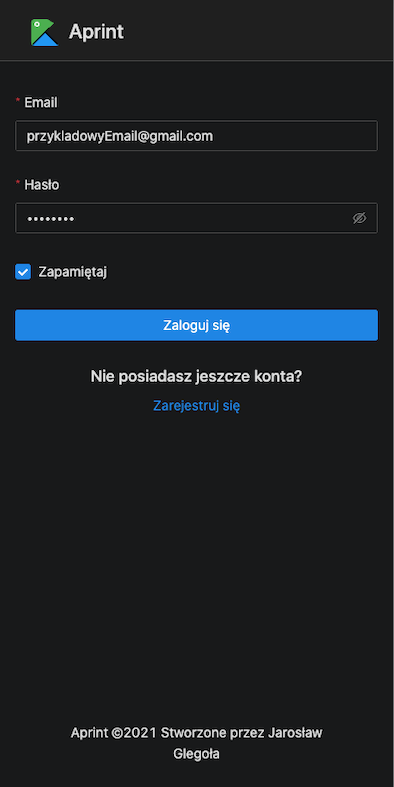
\includegraphics[width=0.45\textwidth]{presentation/login-login.png} }}%
    \qquad
    \subfloat[\centering Krok rejestracji]{{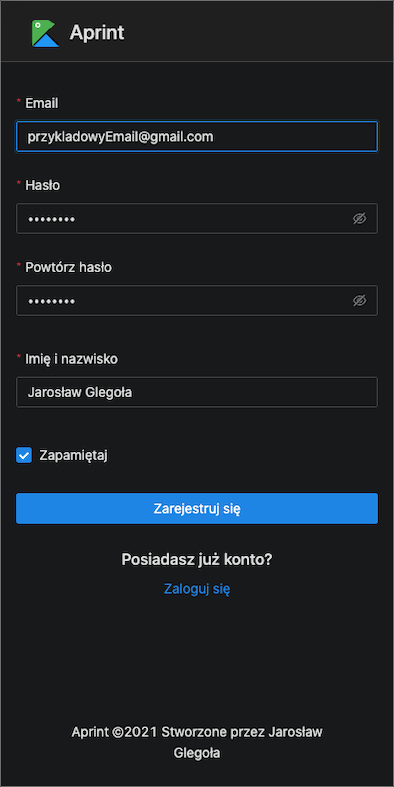
\includegraphics[width=0.45\textwidth]{presentation/login-register.png} }}%
    \caption{Ekran logowania i rejestracji}%
\end{figure}

\clearpage
\subsection{Wydatki}
\subsubsection{Ekran listy wydatków}
Na tym ekranie użytkownik ma dostęp do listy wszystkich wydatków, w których uczestniczy. Na górze ekranu widzimy całkowity bilans kwoty, którą powinien zapłacić oraz kwotę, którą powinien otrzymać od innych użytkowników oraz całkowity bilans tych dwóch kwot. Te dwa kafelki są interaktywne i kliknięcie na jeden z nich zmienia listę wydatków. Ta część odpowiada za wymaganie WF10.

Jeżeli zaznaczona jest opcja \emph{Inni są tobie winni}, na liście wydatków pojawiają się wydatki, których inicjatorem był dany użytkownik, a po zmianie na opcję \emph{Ty jesteś winny w sumie} pojawiają się na liście wydatki, w których użytkownik uczestniczy. Domyślnie zakończone wydatki są ukryte, ale użytkownik ma możliwość zaznaczenia opcji \emph{Pokaż zakończone}, która pokazuje wszystkie wydatki włączając w to te zakończone.

\begin{figure}[h]%
    \centering
    \subfloat{{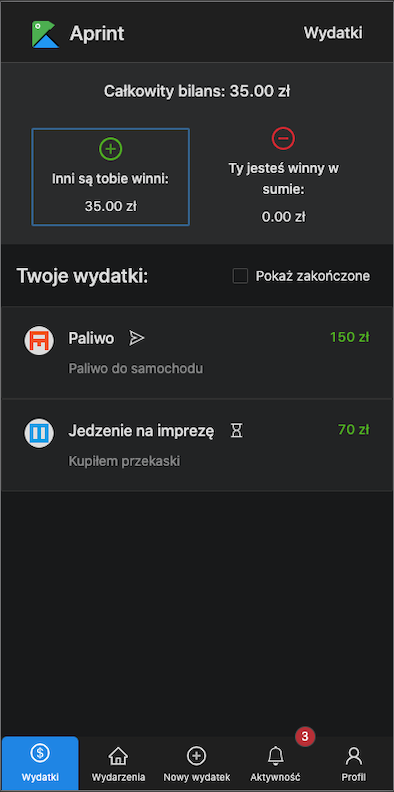
\includegraphics[width=0.45\textwidth]{presentation/responsive-sm.png} }}%
    \caption{Ekran listy wydatków}%
\end{figure}

\clearpage
\subsubsection{Ekran wydatku}
Na ekranie wydatku są ukazane tylko jego dane. Na ekranie jest też pokazany aktualny stan wydatku na komponencie zwanym \emph{krokami}. Dzięki temu komponentowi stan wydatku jest bardziej zrozumiały dla użytkownika. Dodatkowo są też ukazani uczestnicy oraz wszystkie płatności stworzone w ramach wydatku. Inicjator wydatku może z tego poziomu zarządzać wydatkiem, czyli akceptować płatności oraz może zakończyć wydatek. Z tego poziomu może też przejść do ekranu formularza edycji wydatku.

\begin{figure}[h!]%
    \centering
    \subfloat[\centering Wydatek w stanie oczekującym]{{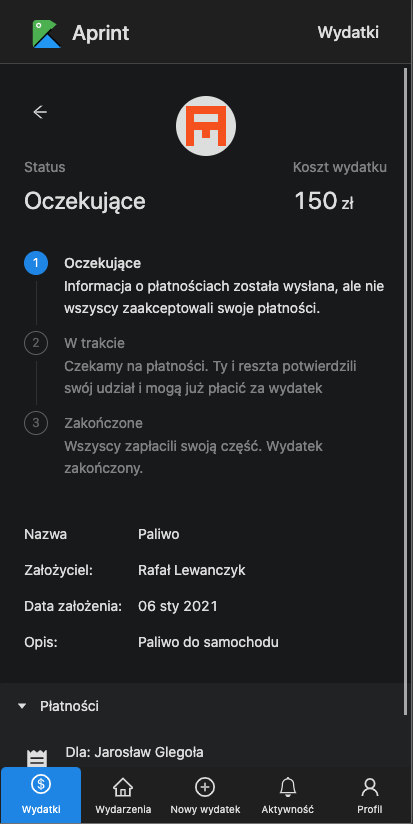
\includegraphics[width=0.31\textwidth]{presentation/expense-waiting.png} }}%
    \qquad
    \subfloat[\centering Wydatek rozpoczęty]{{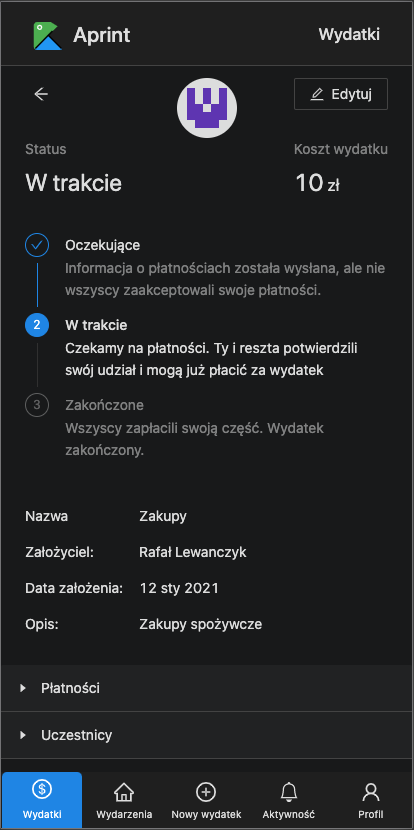
\includegraphics[width=0.31\textwidth]{presentation/expense-in-progress.png} }}%
    \qquad
    \subfloat[\centering Wydatek zakończony]{{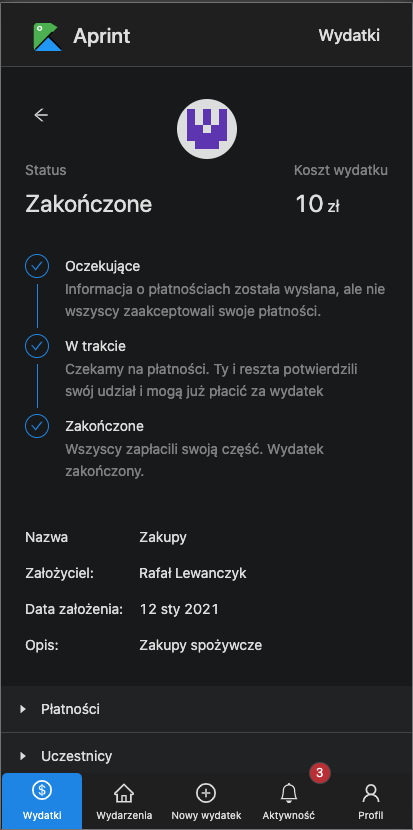
\includegraphics[width=0.31\textwidth]{presentation/expense-ended.png} }}%
    \qquad
    \subfloat[\centering Widok płatności i uczestników wydatku]{{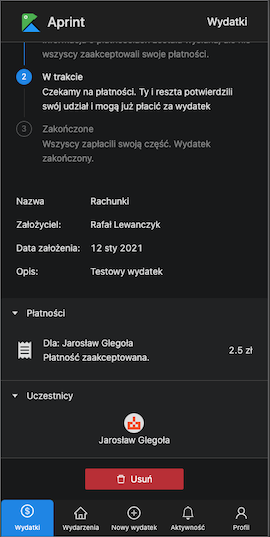
\includegraphics[width=0.31\textwidth]{presentation/expense-bottom-view.png} }}%
    \caption{Ekrany wydatku}%
\end{figure}

\clearpage
\subsubsection{Formularz wydatku}
Ekran tworzenia wydatku pozwala na tworzenie nowych wydatków oraz ich edycji. Wydatki możemy tworzyć dla wydarzeń, grup lub wybierając tylko znajomych. Dane dla każdego typu wydatku się różnią, więc formularz będzie wyglądał inaczej dla każdego typu. Ten formularz spełnia wymaganie WF4 oraz WF7.


\begin{figure}[h!]%
    \centering
    \subfloat[\centering Formularz wydatku w dla wydarzenia]{{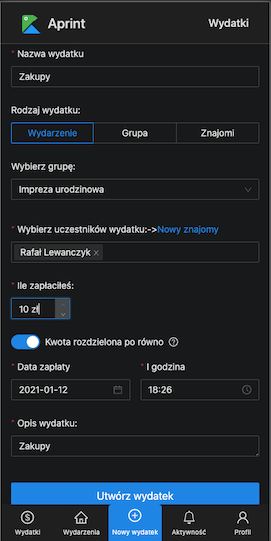
\includegraphics[width=0.31\textwidth]{presentation/expense-form-event.png} }}%
    \qquad
    \subfloat[\centering Formularz wydatku dla grupy]{{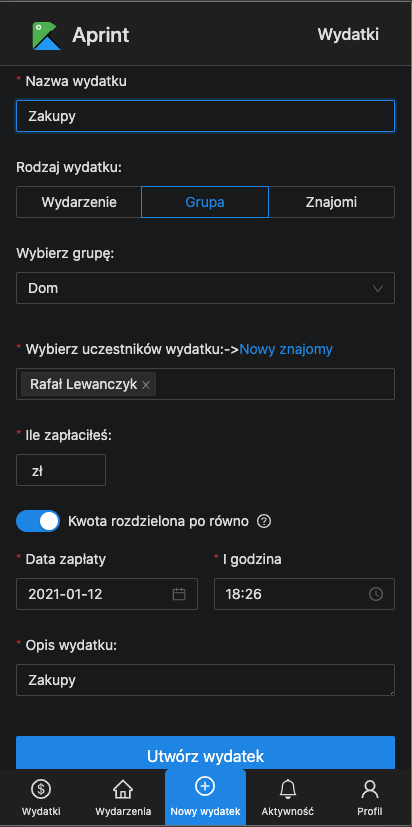
\includegraphics[width=0.31\textwidth]{presentation/expense-form-group.png} }}%
    \qquad
    \subfloat[\centering Formularz wydatku dla znajomych]{{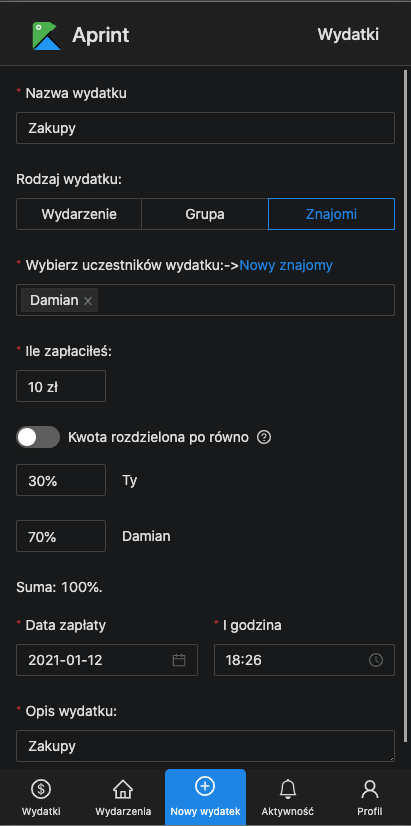
\includegraphics[width=0.31\textwidth]{presentation/expense-form-friends.png} }}%
    \caption{Formularz wydatku}%
\end{figure}

\clearpage
\subsection{Ekran płatności}
Gdy użytkownik zostanie zaproszony do wydatku tworzony zostaje dla niego obiekt płatności, który jest przedstawiony na ekranie płatności. Na tym ekranie są zawarte informacje wydatku, do którego należy płatność, oraz informacje o samej płatności. Z poziomu tego ekranu użytkownik może też zarządzać stanem swojej płatności, czyli akceptować płatność, potwierdzać wpłatę lub odrzucać płatność. Ekran spełnia wymaganie WF5.

\begin{figure}[h!]%
    \centering
    \subfloat[\centering Płatność niepotwierdzona]{{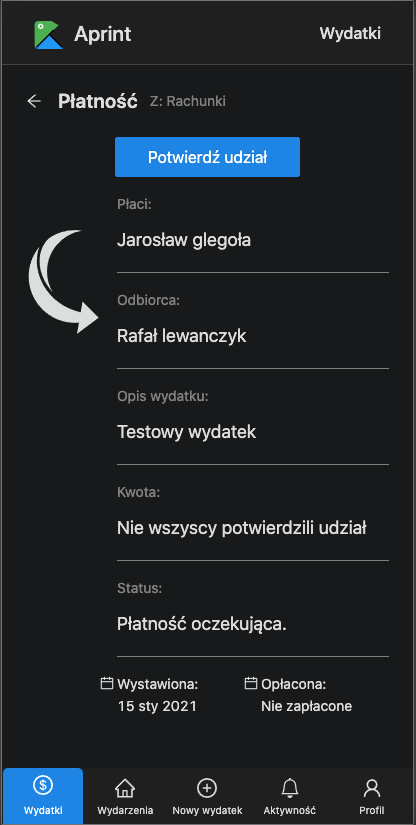
\includegraphics[width=0.31\textwidth]{presentation/payment-to-confirm.png} }}%
    \qquad
    \subfloat[\centering Potwierdzanie płatności]{{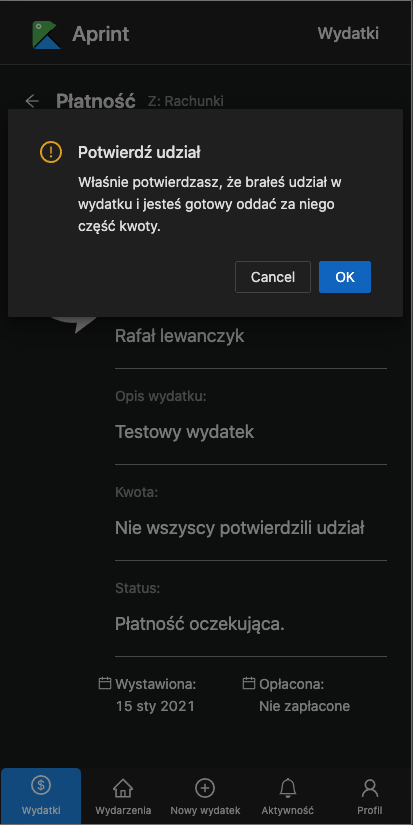
\includegraphics[width=0.31\textwidth]{presentation/payment-confirmation.png} }}%
    \qquad
    \subfloat[\centering Płatność potwierdzona]{{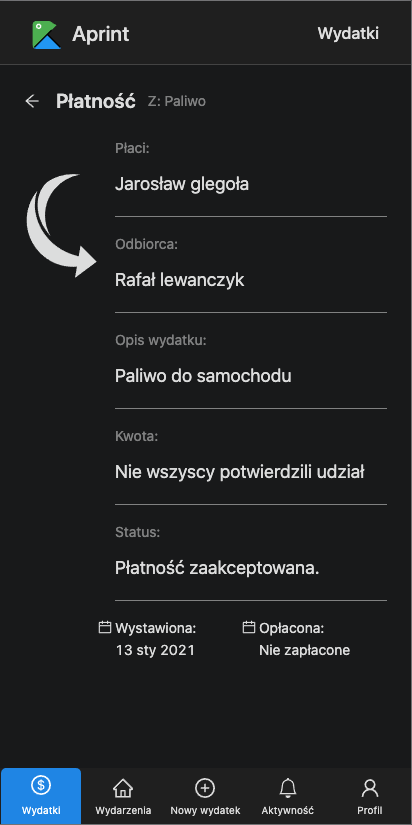
\includegraphics[width=0.31\textwidth]{presentation/payment-confirmed.png} }}%
    \qquad
    \subfloat[\centering Płatność gotowa do zapłaty]{{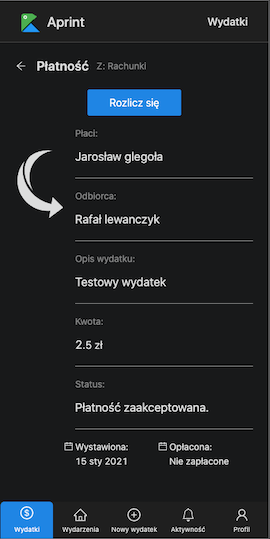
\includegraphics[width=0.31\textwidth]{presentation/payment-to-pay.png} }}%
    \caption{Ekran płatności}%
\end{figure}

\clearpage
\subsection{Ekran wydarzeń, grup i grup znajomych}
\subsubsection{Listy wydarzeń, grup i grup znajomych}
Na głównym ekranie list znajdują się zakładki, dzięki którym użytkownik może wybrać typ elementu. Na tym ekranie mogą pojawić się listy wydarzeń, grup, grup znajomych i zaproszeń. Po kliknięciu na każdy element listy możemy przejść na ekran pojedynczego elementu.

\begin{figure}[h!]%
    \centering
    \subfloat[\centering Lista wydarzeń]{{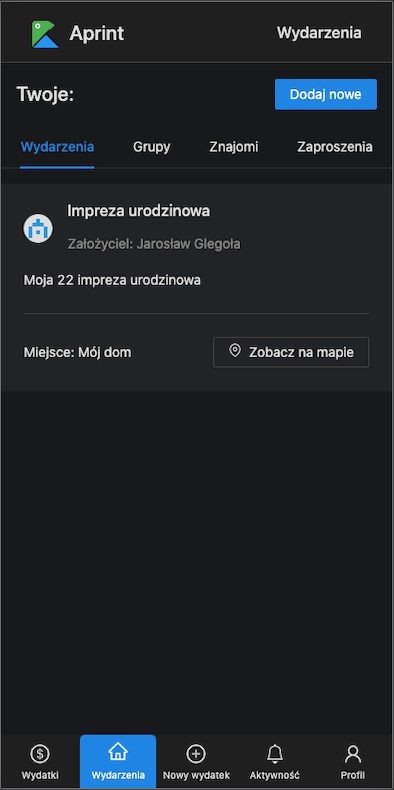
\includegraphics[width=0.45\textwidth]{presentation/event-event-list.png} }}%
    \qquad
    \subfloat[\centering Lista grup]{{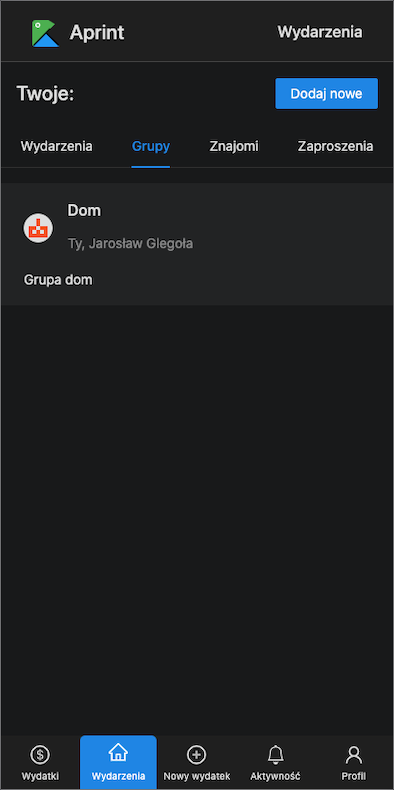
\includegraphics[width=0.45\textwidth]{presentation/event-group-list.png} }}%
    \caption{Listy wydarzeń i grup}%
\end{figure}

\clearpage
\subsubsection{Ekrany wydarzeń, grup i grup znajomych}
Poniżej ukazane są zrzuty ekranu widoków pojedynczych wydarzeń i grup. Na tym widoku są ukazane informacje na temat elementu, lista wydatków oraz wszyscy uczestnicy. Użytkownik z tego poziomu może dołączyć do elementu klikając przycisk \emph{wezmę udział}, gdy użytkownik jeszcze nie zaakceptował zaproszenia, lub opuścić wydarzenie klikając ten sam przycisk, gdy zaproszenie już zaakceptował. Ekran spełnia wymaganie WF6.

Inicjator z tego poziomu może dodawać nowych uczestników, usuwać użytkowników z elementu oraz usuwać dany element.

\begin{figure}[h!]%
    \centering
    \subfloat[\centering Ekran wydarzenia]{{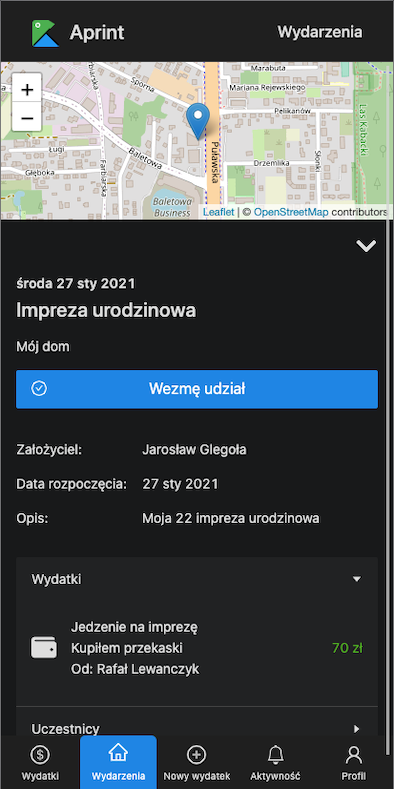
\includegraphics[width=0.45\textwidth]{presentation/event-event-view.png} }}%
    \qquad
    \subfloat[\centering Ekran grupy]{{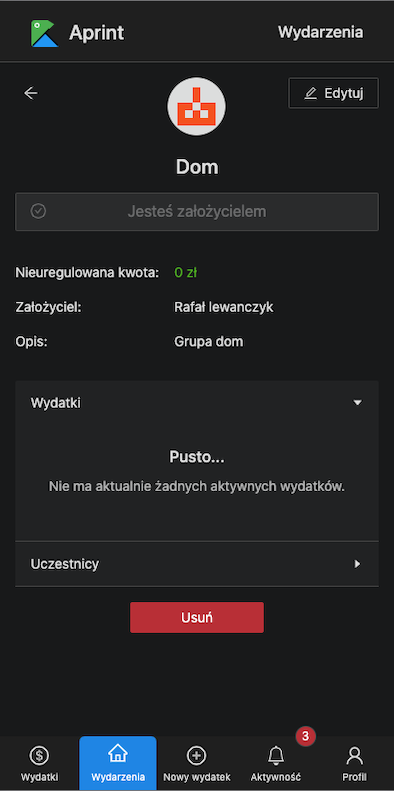
\includegraphics[width=0.45\textwidth]{presentation/event-group-view.png} }}%
    \caption{Ekrany wydarzeń i grup}%
\end{figure}

\clearpage
\subsubsection{Formularz dodawania elementu}
Formularz dodawania elementu umożliwia dodawanie nowego elementu oraz edycję już utworzonego elementu. Formularz może być wyświetlany w dwóch trybach: \emph{Wydarzenie} oraz \emph{Grupa}. W trybie \emph{wydarzenie} mamy możliwość dodania wydarzenia posiadającego datę rozpoczęcia, miejsca wydarzenia oraz możliwości wyboru miejsca na mapie. W trybie \emph{Grupa} mamy możliwość dodania tylko nazwy uczestników i opisu.

\begin{figure}[h!]%
    \centering
    \subfloat{{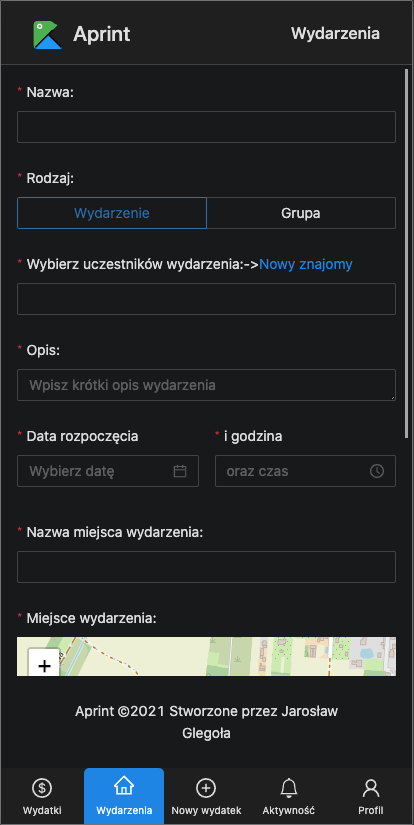
\includegraphics[width=0.31\textwidth]{presentation/event-form-p1.png} }}%
    \qquad
    \subfloat{{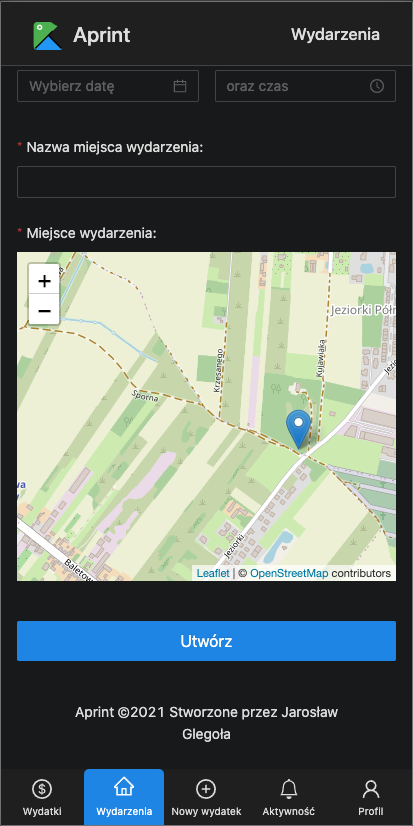
\includegraphics[width=0.31\textwidth]{presentation/event-form-p2.png} }}%
    \caption{Formularz w trybie typu \emph{Wydarzenie}}%
\end{figure}

\begin{figure}[h!]%
    \centering
    \subfloat{{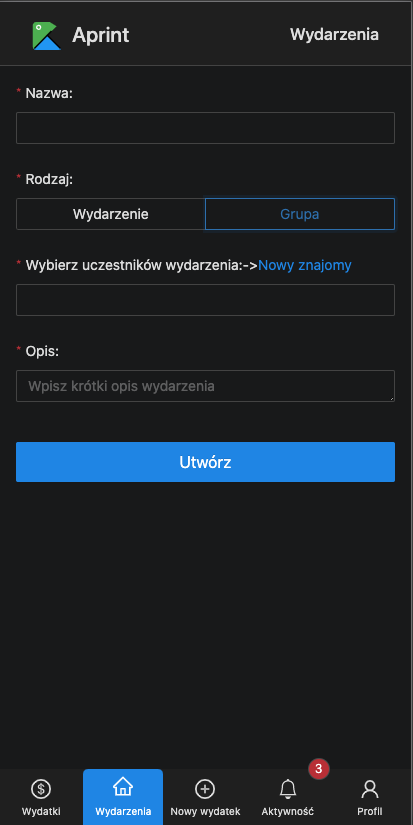
\includegraphics[width=0.45\textwidth]{presentation/event-group-form.png} }}%
    \caption{Formularz w trybie typu \emph{Grupa}}
\end{figure}

\clearpage
\subsection{Aktywność}
Panel aktywności wyświetla użytkownikowi wszystkie dostępne powiadomienia w formie listy. Po kliknięciu w elementy aplikacja przekieruje użytkownika do odpowiednich stron np. po kliknięciu w pierwszy element ukazany na rysunku ~\ref{fig:notificationList} zostaniemy przekierowywani do wydatku, do którego użytkownik został dołączony. Dodatkowo, gdy są na ekranie nowe powiadomienia, wyświetlają się przy nich czerwone kropki, aby zwrócić na nie uwagę użytkownika (przykład na rysunku ~\ref{fig:notificationListNew}). Każde powiadomienie może być usunięte przez użytkownika. Powiadomienia są posortowane w taki sposób, aby najnowsze pojawiały się na samej górze ekranu. Ekran spełnia wymaganie WF8.

\begin{figure}[h!]%
    \centering
    \subfloat[\centering Lista aktywności]{{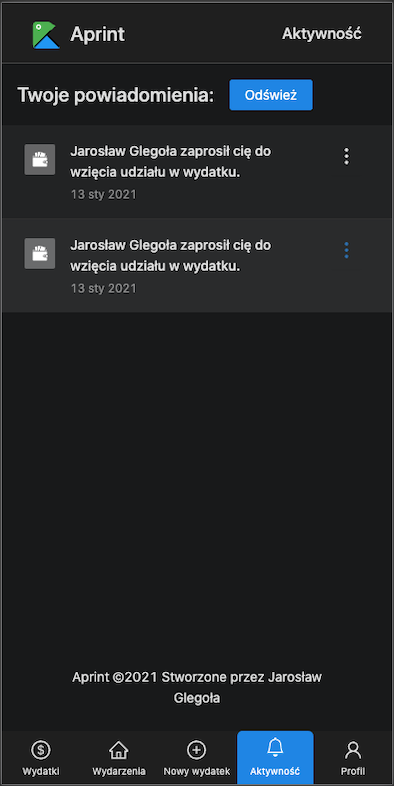
\includegraphics[width=0.45\textwidth]{presentation/notification-list.png} \label{fig:notificationList} }}%
    \qquad
    \subfloat[\centering Lista aktywności z nowym powiadomieniem]{{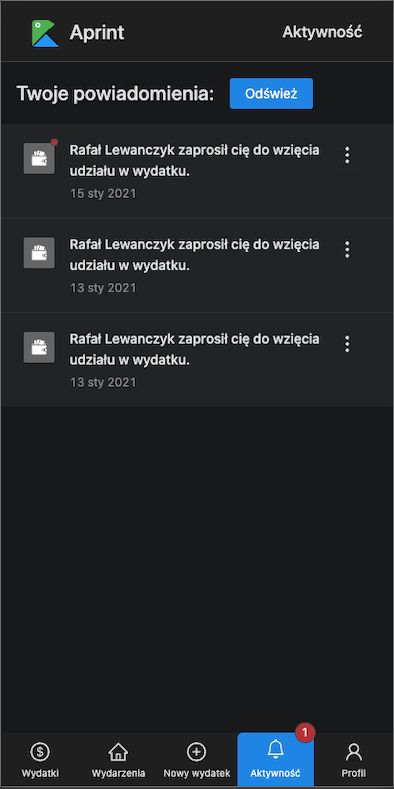
\includegraphics[width=0.45\textwidth]{presentation/notification-list-new.png} \label{fig:notificationListNew}}}%
    \caption{Ekran listy powiadomień}%
\end{figure}

\clearpage
\subsection{Ekrany użytkownika}
\subsubsection{Ekran informacji o użytkowniku}
Na ekranie użytkownika są wyświetlone dane użytkownika tj. imię, numer konta, email. Z poziomu tego ekranu użytkownik może edytować te informacje oraz wylogować się z konta.

\begin{figure}[h!]%
    \centering
    \subfloat[\centering Informacje użytkownika]{{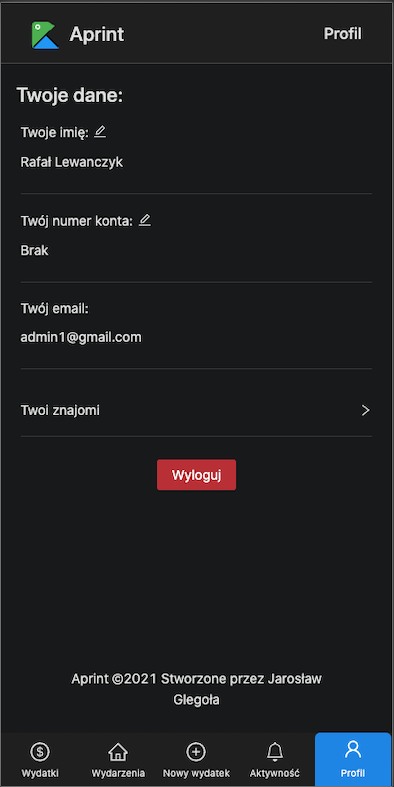
\includegraphics[width=0.45\textwidth]{presentation/user-profile.png} }}%
    \qquad
    \subfloat[\centering Edycja numeru konta]{{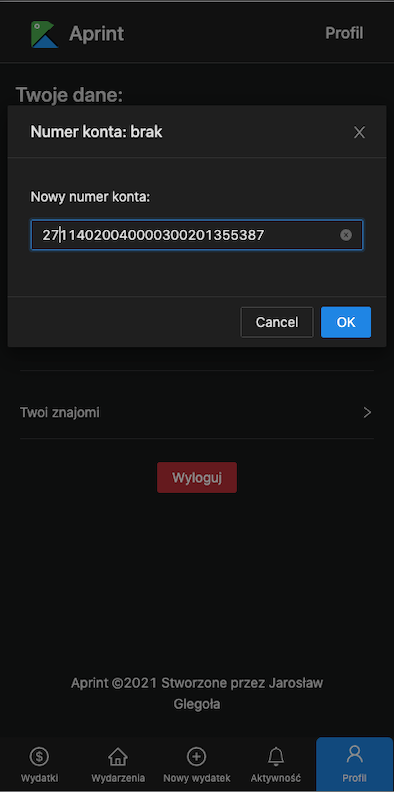
\includegraphics[width=0.45\textwidth]{presentation/user-change-number.png}}}%
    \caption{Ekran użytkownika}%
\end{figure}

\clearpage
\subsubsection{Ekran znajomych}
Na ekranie znajomych znajduje się lista wszystkich znajomych użytkownika oraz mechanizm dodawania nowych użytkowników. Dodatkowo z tego poziomu użytkownik może też usuwać innych użytkowników z listy swoich znajomych. Ekran spełnia wymaganie WF3.

\begin{figure}[h!]%
    \centering
    \subfloat[\centering Lista znajomych]{{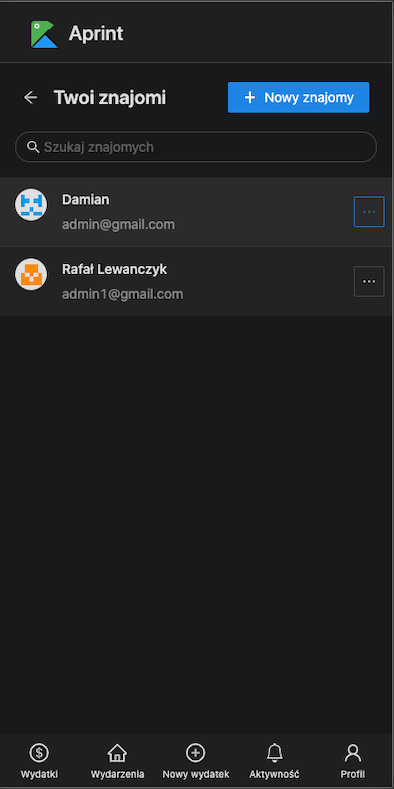
\includegraphics[width=0.45\textwidth]{presentation/friend-list.png} }}%
    \qquad
    \subfloat[\centering Dialog dodawania nowych znajomych]{{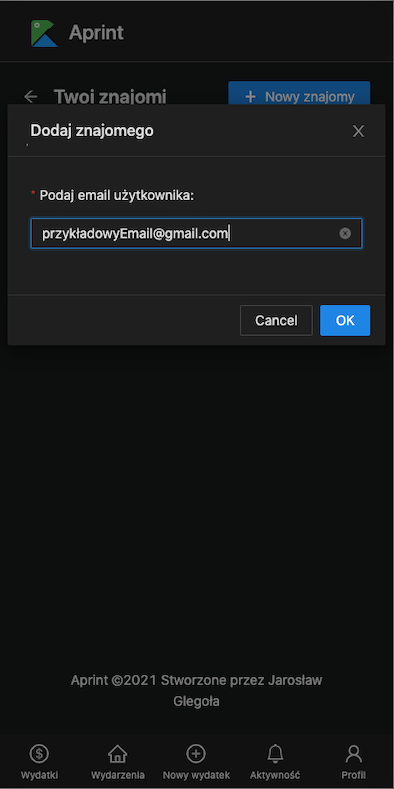
\includegraphics[width=0.45\textwidth]{presentation/friend-add.png}}}%
    \caption{Ekran znajomych}%
\end{figure}

\clearpage
\subsubsection{Ekran innego użytkownika}
Użytkownik może też zobaczyć informacje o innym użytkowniku: jego email, imie oraz numer konta, na który może przelać pieniądze za płatność. Na tym ekranie dostępne są też informacje o balansie pieniężnym pomiędzy użytkownikami. Ekran spełnia wymaganie WF11.

\begin{figure}[h!]%
    \centering
    \subfloat[\centering Lista znajomych]{{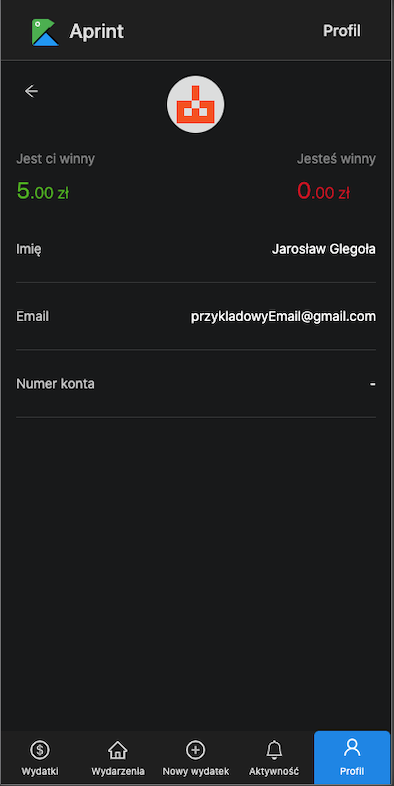
\includegraphics[width=0.45\textwidth]{presentation/friend-view.png} }}%
\end{figure}
